% \subsection{Combining  }

% \textbf{Majority voting only improves accuracy for simpler tasks.} Our experimental results indicate that majority voting enhances accuracy solely when applied to simple questions, and it does not outperform the best individual LLM prediction for complex problems. Through detailed analysis, we observed that for simpler questions, disagreements among individual LLM predictions are typically limited, whereas for complex problems, such disagreements become significantly pronounced. We model this problem by assuming each LLM independently generates answers, where each answer has a probability \( p \) of being correct. Under this assumption, the theoretical accuracy \( A(N, p) \) achievable by majority voting among \( N \) independently predicting models is described by the cumulative probability of a binomial distribution:

% \begin{equation}
% A(N, p) = \Pr\left(X \ge \left\lceil \frac{N}{2} \right\rceil\right) = \sum_{k=\lceil \frac{N}{2} \rceil}^{N} \binom{N}{k} p^{k}(1 - p)^{N - k}, \quad X \sim \text{Binomial}(N, p)
% \end{equation}

% In Figure~\ref{fig:composed_accuracy}, we plot the theoretical accuracy \( A(N, p) \) as a function of individual accuracy \( p \) for different numbers of models (\( N = 3, 5, 7, 9 \)). This plot clearly demonstrates that composed accuracy \( A(N, p) \) surpasses individual accuracy \( p \) only when \( p > 0.5 \). Conversely, for values of \( p \leq 0.5 \), majority voting negatively impacts performance, indicating that aggregation is counterproductive when individual models perform near or below chance.


% \begin{figure}[h]
% \centering
% 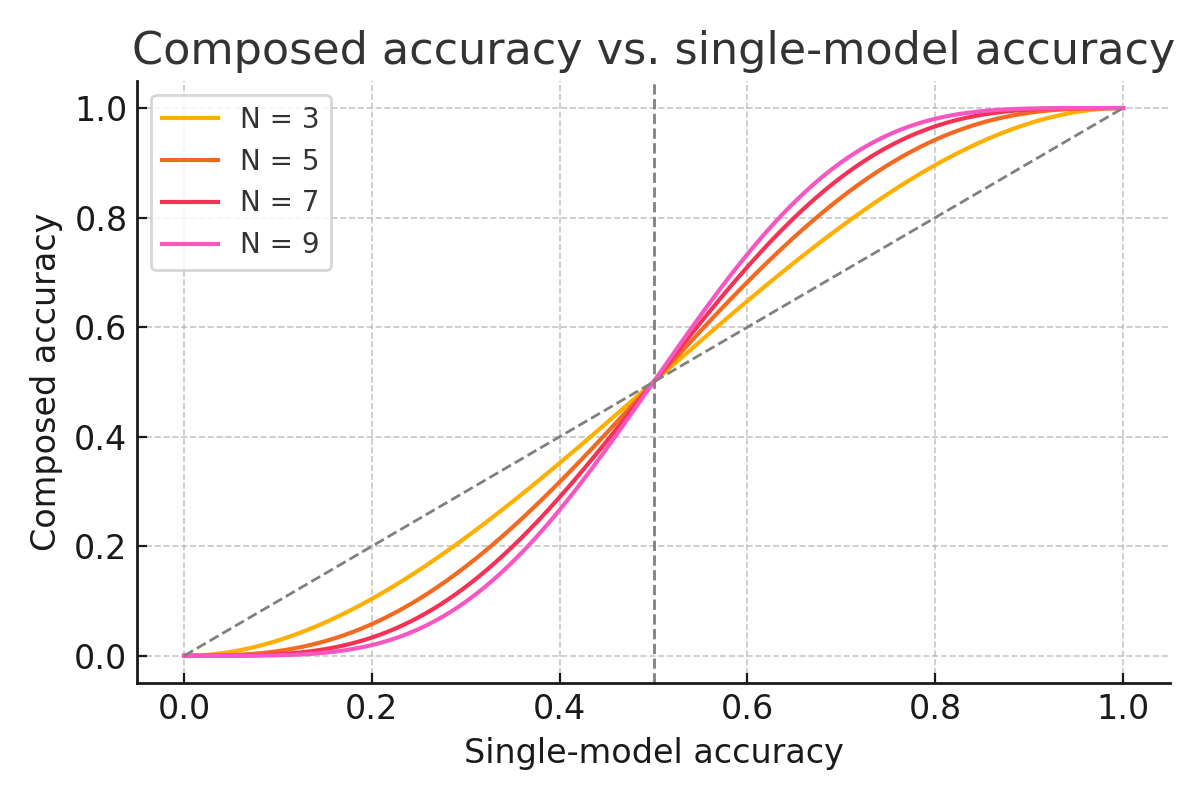
\includegraphics[width=0.7\textwidth]{Figures/majority_accuracy.png}
% \caption{Theoretical analysis of composed accuracy vs. single-model accuracy for different numbers of models $N$.}
% \label{fig:composed_accuracy}
% \end{figure}

% Inspired by this

% Algorithm~\ref{alg:adaptive-routing} formally outlines this adaptive routing procedure:

% \begin{algorithm}[h]
% \caption{Adaptive Routing for Compositional LLMs}
% \label{alg:adaptive-routing}
% \textbf{Input}: Models \( M_1,\dots,M_n \), query \( x \), complex compositional method \( C \), threshold \( 0.5 \) \\
% \textbf{Output}: Final answer \( \hat{y} \)
% \begin{algorithmic}[1]
% \For{\( i=1,\dots,n \)}
%     \State \( y_i \leftarrow M_i(x) \) \Comment{initial independent predictions}
% \EndFor
% \State Compute \( n^* = \max_{y}\sum_{i=1}^{n}\mathbf{1}(y_i = y) \) \Comment{number of majority votes}
% \State Set hyperparameter \(\alpha=1\) for uniform smoothing
% \State Estimate correctness probability \( \hat{p} = \frac{n^*+\alpha}{n+2\alpha} \) via Beta posterior
% \If{\( \hat{p} > 0.5 \)}
%     \State \( \hat{y} \leftarrow \) majority vote over predictions \( y_i \) \Comment{simple aggregation}
% \Else
%     \State \( \hat{y} \leftarrow C(M_1,\dots,M_n, x) \) \Comment{advanced compositional method}
% \EndIf
% \State \textbf{return} \( \hat{y} \)
% \end{algorithmic}
% \end{algorithm}






